\documentclass{abnt}
\usepackage[utf8]{inputenc}
\usepackage[num]{abntcite}
\usepackage{graphicx}
\usepackage{url}
\usepackage{caption}
\usepackage{listings}
\usepackage[brazil]{babel}

\lstset{
  basicstyle=\small\sffamily,
  numbers=left,
  numberstyle=\tiny,
  frame=tb,
  columns=fullflexible,
  showstringspaces=false
}

\graphicspath{{imagens/}}

\begin{document}
\autor{André Taiar Marinho Oliveira}

\titulo{Sistema para construção de bibliotecas virtuais de compostos químicos}

\orientador[Orientadora:\\]{Profa. Dra. Rafaela Salgado Ferreira}
\coorientador[Orientadora:\\]{Profa. Dra. Raquel Cardoso de Melo Minardi}

\comentario{Apresentado como requisito da disciplina de Atividades Práticas Integradoras - DCC/UFMG}

\instituicao{Universidade Federal de Minas Gerais \par Instituto de Ciências
Exatas \par Departamento de Ciência da Computação}

\local{Belo Horizonte} \data{2016/2}

\capa
\folhaderosto

\begin{resumo}
Com o crescimento e disseminação da quimioinformática, experimentos \textit{in silico}
(análises feitas através de simulação computacional) surgem como opções que economizam
diversos recursos e tempo de pesquisadores em processos laboratoriais na obtenção
de compostos. Algumas ferramentas entretanto são comerciais e muito caras para que
grande parte dos laboratórios tenham acesso a suas funcionalidades. Neste trabalho
foi desenvolvido uma ferramenta que permite a filtragem de reagentes químicos disponíveis
em bases de moléculas comercialmente disponíveis e a combinação entre tais moléculas
através de reações químicas, gerando uma biblioteca virtual de compostos químicos.
Tal sistema foi desenvolvido em ambiente web e está disponível gratuitamente para
uso geral.\\

\textbf{Keywords}: quimioinformática, sistemas web, bibliotecas, compostos, reações.
\end{resumo}

\sumario
\listoffigures

\chapter{Introdução}

\section{Visão geral do assunto}

A Quimioinformática é uma área interdisciplinar que trabalha a modelagem e resolução
de problemas químicos utilizando infraestrutura computacional. Neste trabalho iremos
utilizar diversas ferramentas e técnicas da quimioinformática para resolver um problema
de química combinatória. Combinamos através de experimentos \textit{in silico} bases de
reagentes químicos através de simulações de reações químicas gerando bibliotecas
de compostos químicos para serem analisadas posteriormente.

\section{Objetivo, justificativa e motivação}

Existem ferramentas comerciais que realizam, em partes, o trabalho que estamos propondo.
Tais ferramentas, porém, tem um alto custo e licenças que os tornam inacessíveis
para grande parte dos laboratórios e usuários que trabalham na área. Iremos desenvolver
a solução em formato de sistema web e disponibilizá-la gratuitamente na internet
para uso e colaboração no crescimento deste sistema. Pelo potencial desta aplicação
em ajudar outros laboratórios e cientistas, já existem ações em andamento para que
ele continue sendo mantido e expandido. De qualquer forma, o protótipo inicial foi
completamente projetado e desenvolvido neste trabalho.

\chapter{Contextualização e trabalhos relacionados}

A Quimioinformática\cite{brown1998chemoinformatics} é uma área interdisciplinar que envolve a Química e a Informática
e consiste no uso de técnicas computacionais aplicadas a uma gama de problemas no
campo da Química. Dentre suas utilizações mais básicas estão o armazenamento, indexação,
busca de informações relativas a compostos químicos, representação de átomos, moléculas
e reações químicas entre moléculas, bases e bibliotecas de compostos químicos e
recuperação de informação nestas bases. A Quimioinformática é sistematicamente utilizada
para análise \textit{in silico} (análises feitas através de simulação computacional) nas
indústrias farmacêuticas, na Bioinformática e em qualquer laboratório de Química
atualmente.

A Química Combinatória\cite{RBCF43904} é uma grande ferramenta para a descoberta e o desenvolvimento
de novos compostos químicos de interesse em diversas áreas. Nesta metodologia de
síntese os produtos são formados simultaneamente através da combinação de diversos
compostos e os experimentos são analisados depois de gerados. A principal meta desta
metodologia é reduzir o tempo necessário para, por exemplo, a obtenção de um novo
fármaco. É fácil perceber que na abordagem combinatorial gasta-se tempo na composição
de uma quimioteca (uma biblioteca de experimentos já verificados de forma combinatória)
bem como gastam-se compostos químicos que nem sempre serão utilizados em sua totalidade
ou mesmo irão gerar um resultado de interesse para a análise final.

Com a popularização e uma maior utilização da computação e da Quimioinformática,
é possível reduzir o tempo gasto e a utilização de compostos em experimentos combinatoriais.
Utilizando bases pré-definidas de reagentes, preparadas e filtradas arbitrariamente
e combinando tais reagentes através de uma reação química conhecida, podemos observar
as características dos compostos resultantes e obter uma boa aproximação do que
aconteceria com os experimentos na realidade.

Neste trabalho, foi desenvolvido um sistema computacional com interface web que
permite a busca por reagentes de interesse em bases de compostos químicos através
de diversos filtros de propriedades de moléculas. A partir desta busca, o usuário
terá uma visualização dos resultados obtidos e a possibilidade de reagir quimicamente
os compostos encontrados na busca, obtendo ao final os dados de todos os compostos
possíveis gerados a partir da reação química entre todas as combinações encontradas
nas bases filtradas. Estes resultados são automaticamente exportados em um formato
de planilha eletrônica, contendo a biblioteca gerada e permitindo salvar a informação
e fazer futuras análises com os experimentos gerados.

Em nosso protótipo utilizamos uma base de reagentes da Sigma-Aldrich\cite{SIGMA} que é uma grande
empresa norte americana do ramo da química, biotecnologia e ciências da vida. Essa
empresa é um conceituado fornecedor de compostos químicos para laboratórios de todo
o mundo. Seu catálogo é fornecido em diversos formatos pelo ZINC\cite{ZINC} que é uma base de
dados (não comerciais) de compostos químicos comercialmente disponíveis, além de
uma infinidade de outras funcionalidades ligadas à Bioinformática e farmacêutica.
O ZINC é uma ferramenta gratuita desenvolvida e fornecida por laboratórios do Departamento
de Química Farmacêutica da Universidade da Califórnia, em São Francisco (UCSF),
EUA \cite{UCSFCHEM}.

Foram utilizadas muitas ferramentas, todas disponíveis gratuitamente, na composição
do sistema desenvolvido. Dentre as que compõem o back-end do projeto, a mais importante
é o Open Babel\cite{OPEN_BABEL}. Segundo palavras do próprio site o Open Babel é um conjunto de ferramentas
projetado para lidar com as muitas linguagens dos dados químicos. No sistema ele
é responsável por ler as bases de reagentes (disponibilizados em um formato bem
específico para moléculas) e buscar os componentes, converter formatos de dados
químicos, extrair informações das moléculas e até mesmo gerar a visualização em
imagem das moléculas para a web.

Todas as moléculas no sistema são representadas por meio de uma notação chamada
SMILES (\textit{Simplified Molecular Input Line Entry System})\cite{DL_SMILES}. Esta notação foi criada
por uma empresa chamada Daylight, que também é uma referência na produção de sistemas
químicos. Para procurar por determinados padrões e características nas moléculas,
utilizamos uma linguagem, também criada pela Daylight, chamada SMARTS\cite{DL_SMARTS}. A mesma empresa
também fornece uma linguagem para descrição de reações e transformações químicas
chamada SMIRKS\cite{DL_SMIRKS}. Apesar disso, para as reações em nosso sistema não utilizamos os
SMIRKS mas sim, uma outra linguagem chamada Reaction SMARTS. Essa linguagem basicamente
usa SMARTS para descrever uma transformação química. Para executar a reação química
utilizamos uma outra ferramenta livre chamada RDKit\cite{RDKIT}.

\chapter{Método do trabalho}

Este trabalho foi definitivamente o meu primeiro contato com a Bioinformática durante
toda a graduação e o primeiro passo necessário foi tentar entender bem o problema
que a minha orientadora e idealizadora do projeto, Rafaela Ferreira, me passou em
diversas reuniões que fizemos em seu início. Juntamente com a minha
outra orientadora, Raquel Minardi, aos poucos as funcionalidades necessárias foram
ficando claras finalmente conseguimos definir um escopo.

Desde as reuniões mais iniciais sobre o tema deste trabalho, mesmo antes de entender
corretamente o escopo do projeto, já era determinado que o mesmo deveria ser disponibilizado
em forma de um sistema web por diversos motivos: facilidade para a manutenção em
um lugar centralizado, facilidade para atualização, distribuição e internacionalização
do sistema.

Por uma preferência pessoal de forma de trabalho, foi utilizada uma metodologia
de trabalho muito parecida com metodologias ágeis de desenvolvimento de software\cite{alliance2001agile},
mais especificamente o Scrum\cite{schwaber2011scrum}. Houve a primeira parte do trabalho aonde os requisitos
do projeto foram ficando claros ao longo de diversas reuniões, em um formato de
pré-jogo do Scrum. Nessas reuniões basicamente foram tomadas notas e muito conteúdo
era levado para ser pesquisado e analisado. Houve durante esta etapa do projeto
um trabalho sobre análise de viabilidade, do que era possível ou não fazer dentro
do que foi idealizado inicialmente para o projeto.

Após definido inicialmente o que seria possível fazer dentro do esperado para o
sistema, foram definidas algumas funcionalidades prioritárias iniciais em forma
de um backlog de projeto e gradativamente este backlog foi sendo desenvolvido e
agregado ao projeto principal na forma de Sprints. As Sprints, na maioria das vezes,
duraram 1 semana. Sempre iniciavam com o planejamento das funcionalidades a serem
implementadas para a próxima iteração do projeto. Em seguida, haveria a fase de
desenvolvimento do projeto e, ao final do desenvolvimento, uma reunião de revisão
da Sprint. Nesta eram mostradas as funcionalidades que foram desenvolvidas ao decorrer
da Sprint para a professora Rafaela (que automaticamente tomou um papel de Product
Owner). Então o ciclo se repetia. Ainda sobraram no backlog do produto final entregue
neste trabalho, diversas funcionalidades que ainda são bastante interessantes e muito
trabalho futuro ainda será possível a partir deste trabalho inicial, como descreverei
melhor na conclusão do trabalho.

Acredito que o andamento do trabalho não poderia ter ocorrido de melhor forma, dadas
as dificuldades que tive inicialmente para encontrar as minhas orientadoras e definir
o meu tema. Trabalhar de acordo com metodologias ágeis permitiu que as funcionalidades
prioritárias do sistema fossem desenvolvidas primeiro e que um refinamento progressivo
do que deveria ou não entrar em cada fase do desenvolvimento fosse naturalmente clara
ao longo do processo. O contato periódico com as orientadoras ajudou bastante a
tirar as dúvidas e acelerar o processo de elicitação dos requisitos. Acredito ter
escolhido o método correto para trabalhar nessa situação. O atraso inicial do projeto
provavelmente valeu a pena dado que eu me interessei realmente pelo tema (foi bastante
satisfatório o desenvolvimento do trabalho para mim) e escolhi excelentes orientadoras
que me ajudaram bastante no trabalho e a quem muito agradeço pela atenção e disponibilidade.

\chapter{Desenvolvimento do trabalho}

\section{Definição e requisitos do projeto}

O intuito do projeto é desenvolver uma plataforma gratuita e pública para que usuários
de laboratórios de todo o mundo possam buscar e experimentar reações químicas entre
bases de reagentes moleculares com determinadas características de interesse que
possam ser filtradas. Ao final do processo, uma biblioteca com todas as informações
geradas deve ser exportada em um formato acessível para que o usuário possa analisar
as reações ocorridas e quais compostos são de seu interesse.

Com tais requisitos foi vislumbrado que o ideal seria desenvolver um sistema em
plataforma web, disponível através do browser. A base a ser utilizada seria inicialmente
a base de compostos oferecidos pela empresa Sigma-Aldrich (pela relevância que tal
empresa tem no mercado pela venda de seus reagentes químicos) mas que poderia, futuramente,
ser expandido para a busca de reagentes em diversas bases.

Para selecionar as moléculas de interesse existentes nessa grande base de reagentes
(na base de compostos da Sigma-Aldrich oferecida pelo ZINC e atualizada em 21/04/2015
existem mais de 100.000 compostos) precisamos filtrar segundo alguns critérios de
interesse. O primeiro tipo de critério utilizado para a filtragem nesta base é uma
busca por grupos funcionais. Esta filtragem foi implementada por meio de um casamento
de padrões utilizando SMARTS dos grupos funcionais. A aplicação já provê alguns
SMARTS pré-definidos: Ácido Carboxílico, Amina e Amida, e dá a opção para que o
usuário com conhecimento em SMARTS possa fazer o input de seu SMARTS de interesse.
Uma das melhorias previstas para fazer futuramente é o input do SMARTS através do
desenho da molécula, utilizando alguma ferramenta gráfica que dê suporte a tal funcionalidade.

O segundo tipo de informação que pode ser filtrada dentro das bases de reagentes
tem haver com características específicas de cada molécula. Foram implementados
campos para input de valores mínimos e máximos esperados para cada um dos critérios
filtrados. Os critérios possíveis para filtragem nas moléculas atualmente são: massa
molecular, número de átomos, doadores de ligação de hidrogênio, receptores de ligação
de hidrogênio, número de anéis e LogP. Todos podem ser combinados com suas quantidades
mínimas e máximas esperadas para que o resultado seja refinado arbitrariamente.

É necessário a geração de mais de uma base para que possamos fazer a reação entre
bases diferentes. Atualmente o sistema permite gerarmos apenas duas bases simultaneamente.
Uma das funcionalidades previstas para as próximas versões é permitir a geração
de mais de duas bases através de filtragem e poder reagir todas as bases, gerando
assim ainda mais resultados.

Após a busca nas bases, os resultados dos reagentes encontrados são exibidos. Em
uma tabela são listados os desenhos das moléculas, sua fórmula e todos os critérios
de filtragem citados anteriormente com o valor pertencente a cada uma das moléculas.
Com tais bases geradas, é possível executar a simulação da reação química entre todos
os reagentes pertencentes a cada uma delas. Para isso, basta selecionar a reação
desejada em uma lista de reações já disponíveis na aplicação.

Para executar as reações, utilizamos uma linguagem chamada Reaction SMARTS. Ao contrário
dos SMARTS de busca de padrões nas moléculas que usamos anteriormente, ainda não
disponibilizamos o input de Reaction SMARTS na aplicação pelo usuário (mas isso
está previsto para acontecer posteriormente). Após a seleção da reação e o comando
para executá-la, é gerado um arquivo em formato de planilha eletrônica e automaticamente
é feito o seu download.

Mais resultados e exemplos da utilização do sistema serão vistos no capítulo Resultados
e discussão.

\section{Verificação da viabilidade}

Com os requisitos da aplicação em mãos, precisamos buscar os componentes certos
para compor o trabalho de forma a viabilizar que tudo funcione como planejado. O
primeiro problema resolvido foi a forma de pesquisa na base de dados. O ZINC fornece
as bases que iremos trabalhar em diversos formatos de dados. Os que nos interessam
são os formatos MOL2 e PDB. Estes formatos contém diversas informações sobre as
moléculas já pré-calculadas que serão úteis para a extração de outras informações
necessárias no projeto. O Open Babel é a ferramenta que utilizamos para trabalhar
com estas bases de dados. Por ser uma ferramenta especializada nesse tipo de operações
(trabalhar com dados de bases de dados químicas, conversão dos formatos de arquivos,
busca etc) acabou se tornando o principal componente do back-end em nossa aplicação.

O segundo problema a ser resolvido era a execução das reações. Existem atualmente
boas ferramentas comerciais que realizam reações \textit{in silico} de moléculas mas são
poucas as opções gratuitas que fazem um trabalho satisfatório. A única opção encontrada
e adotada no trabalho até o momento é através do RDKit. Como seu próprio slogan diz,
ele é um programa open source de quimioinformática. O RDKit é uma suíte grande e
completa e com muitas funcionalidades para desenvolver software químico. Neste trabalho,
apenas adaptamos um programa já existente que utiliza o RDKit para executar as reações
e foi fornecido pelo ZINC.

Após resolver estes problemas, tivemos segurança de que o projeto era possível de
ser executado como queríamos e partimos para a implementação da plataforma.

\section{Definição da tecnologia}

Foi escolhido para compor a aplicação a linguagem Ruby com o framework Ruby on Rails
por diversos motivos. Primeiramente, pela facilidade que este traz para escrever
aplicações web de forma rápida e prática. Em segundo lugar, o Open Babel disponibiliza
toda a sua API também para a linguagem Ruby, o que seria essencial para utilizá-lo
como engine de busca e conversões de formatos dentro da aplicação. O RDKit infelizmente
não oferece bindings para linguagem Ruby como o Open Babel, ele oferece suporte
apenas à linguagem Python. Nesse caso, tivemos que trabalhar com chamadas de sistema
diretamente à aplicação que utiliza o RDKit.

\section{Descrição da arquitetura do projeto}

Um diagrama da arquitetura do projeto com os principais componentes do sistema pode
ser visto na figura \ref{fig:arq}.

O framework web Ruby on Rails é o componente do sistema responsável por distribuir
as tarefas aos outros componentes do back-end baseado na interação do usuário. Ele
recebe requisições da internet, as interpreta, aciona os componentes do back-end
e retorna uma resposta ao usuário. Existe uma camada entre o Rails e o Open Babel
chamado Rubabel. Rubabel é uma biblioteca que abstrai alguns conceitos do Open Babel
e os torna mais acessíveis aos usuários da linguagem Ruby. O Open Babel faz comunicação
direta com as bases de reagentes disponíveis na aplicação efetuando as ações necessárias.

Como não existe API direta entre a linguagem Ruby e o RDKit, foi necessário o uso
de chamadas de sistema para comunicação entre o framework Ruby on Rails e uma aplicação
que executa as operações necessárias utilizando o RDKit. Esta aplicação se chama
ZINC Reactor e foi fornecida ao projeto pelo responsável pela aplicação do ZINC.
O ZINC Reactor é a aplicação que faz a combinação entre as moléculas de cada uma
das bases, passando para o RDKit executar a reação entre elas. Ao final, o resultado
das reações é repassado à aplicação Rails para dar continuidade ao processo de exportação.

\begin{figure}[!htb]
  \centering
  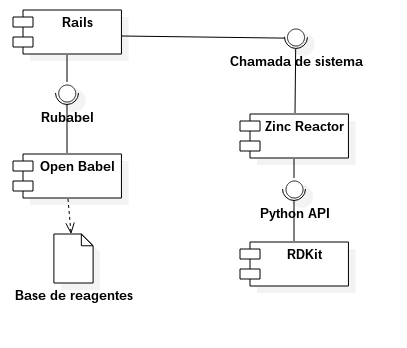
\includegraphics[scale=0.8]{diagrama_de_arquitetura.png}
  \caption{Diagrama de arquitetura do sistema}
  \label{fig:arq}
\end{figure}

\chapter{Resultados e discussão}

Vamos apresentar abaixo um exemplo de utilização do fluxo completo criado na
aplicação. Na figura \ref{fig:react1}, temos a tela inicial da aplicação. Podemos
verificar a presença dos campos de filtragem para as duas bases de dados que iremos
gerar em seguida.

\begin{figure}[!htb]
  \centering
  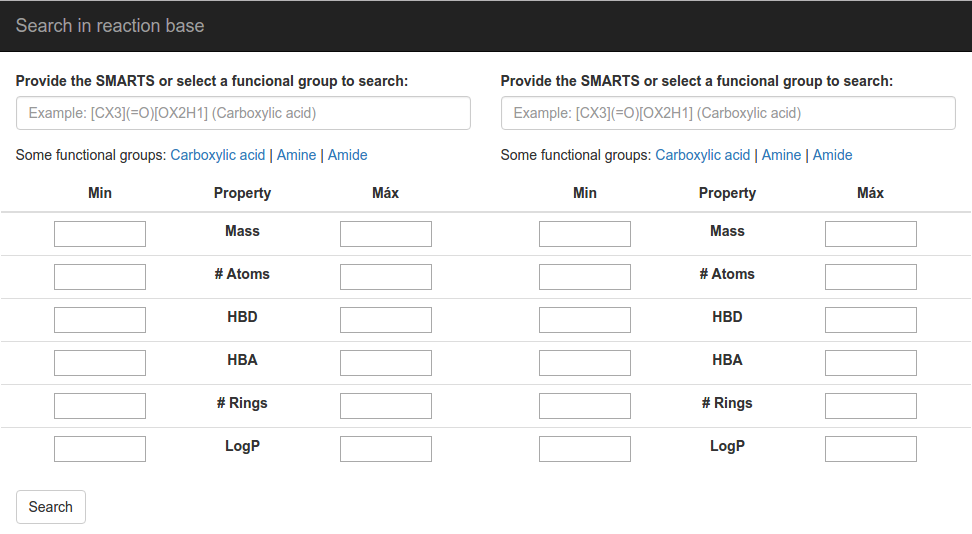
\includegraphics[scale=0.5]{reaction1}
  \caption{Tela inicial ao acessar o sistema.}
  \label{fig:react1}
\end{figure}

Na figura \ref{fig:react2} temos um exemplo do preenchimento de uma das possíveis
filtrages nas bases de dados. Para a Base 1 foi escolhido o grupo funcional Ácido
Carboxílico e um número máximo de 10 átomos presentes nesta molécula. Já para a
Base 2 os filtros foram preenchidos com o grupo funcional da Amina e foi feita uma
filtragem aonde apenas moléculas com pelo menos 120 átomos estarão presentes em
seus resultados.

\begin{figure}[!htb]
  \centering
  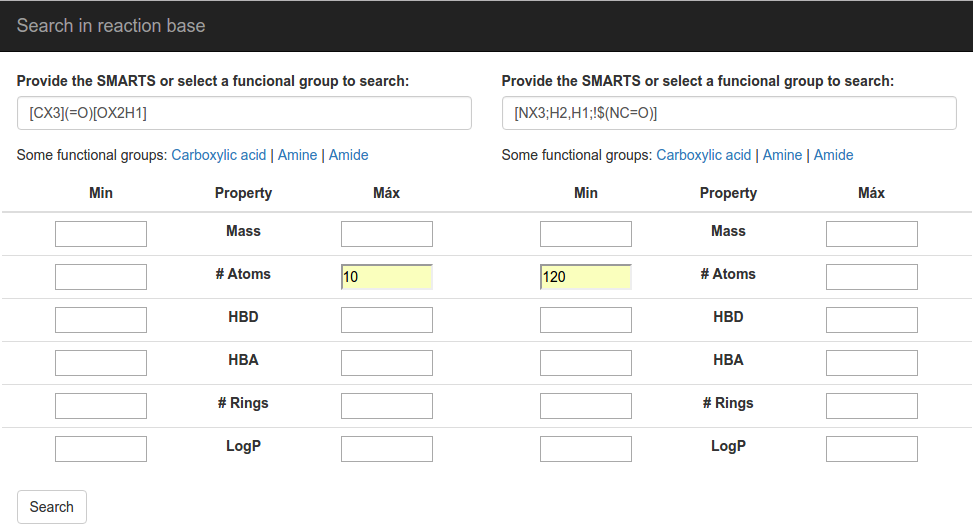
\includegraphics[scale=0.5]{reaction2}
  \caption{Exemplo de preenchimento dos filtros do sistema.}
  \label{fig:react2}
\end{figure}

Após a filtragem das bases clicando no botão de busca, podemos ver na imagem \ref{fig:react3}
um exemplo da exibição dos resultados encontrados de acordo com os filtros para
cada uma das bases. Perceba, por exemplo, que todas as moléculas que aparecem no
detalhe da imagem contém 10 ou menos átomos, o que corresponde à nossa filtragem
na imagem \ref{fig:react2}.

\begin{figure}[!htb]
  \centering
  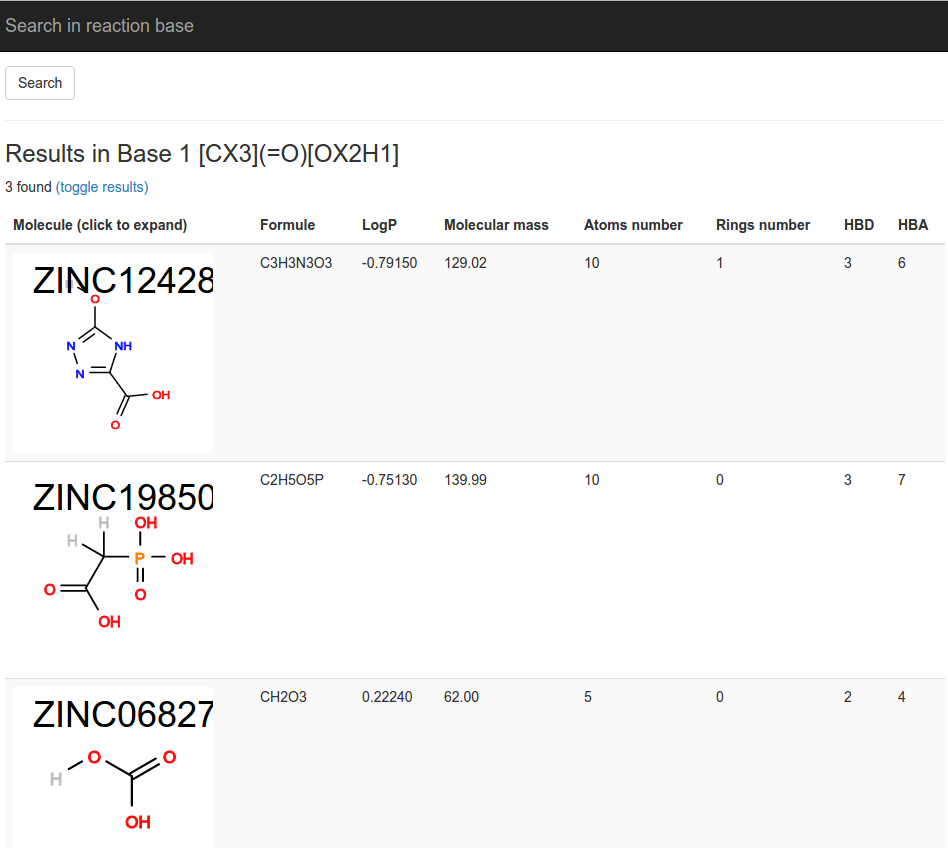
\includegraphics[scale=0.5]{reaction3}
  \caption{Exemplo de resultados da filtragem das bases do sistema.}
  \label{fig:react3}
\end{figure}

Na imagem \ref{fig:react4} podemos ver a seleção da reação química que irá ser executada
entre os reagentes filtrados nas duas bases.

\begin{figure}[!htb]
  \centering
  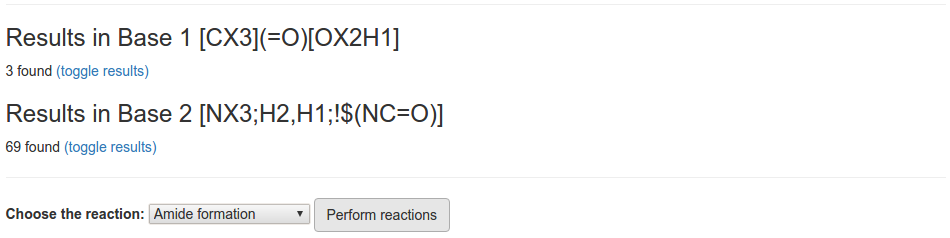
\includegraphics[scale=0.5]{reaction4}
  \caption{Seleção da reação química que irá reagir as duas bases filtradas.}
  \label{fig:react4}
\end{figure}

Finalmente, no detalhe da figura \ref{fig:react5} podemos ver o resultado da exportação
ocorrido ao final de todas as reações em um programa de planilha eletrônica.

\begin{figure}[!htb]
  \centering
  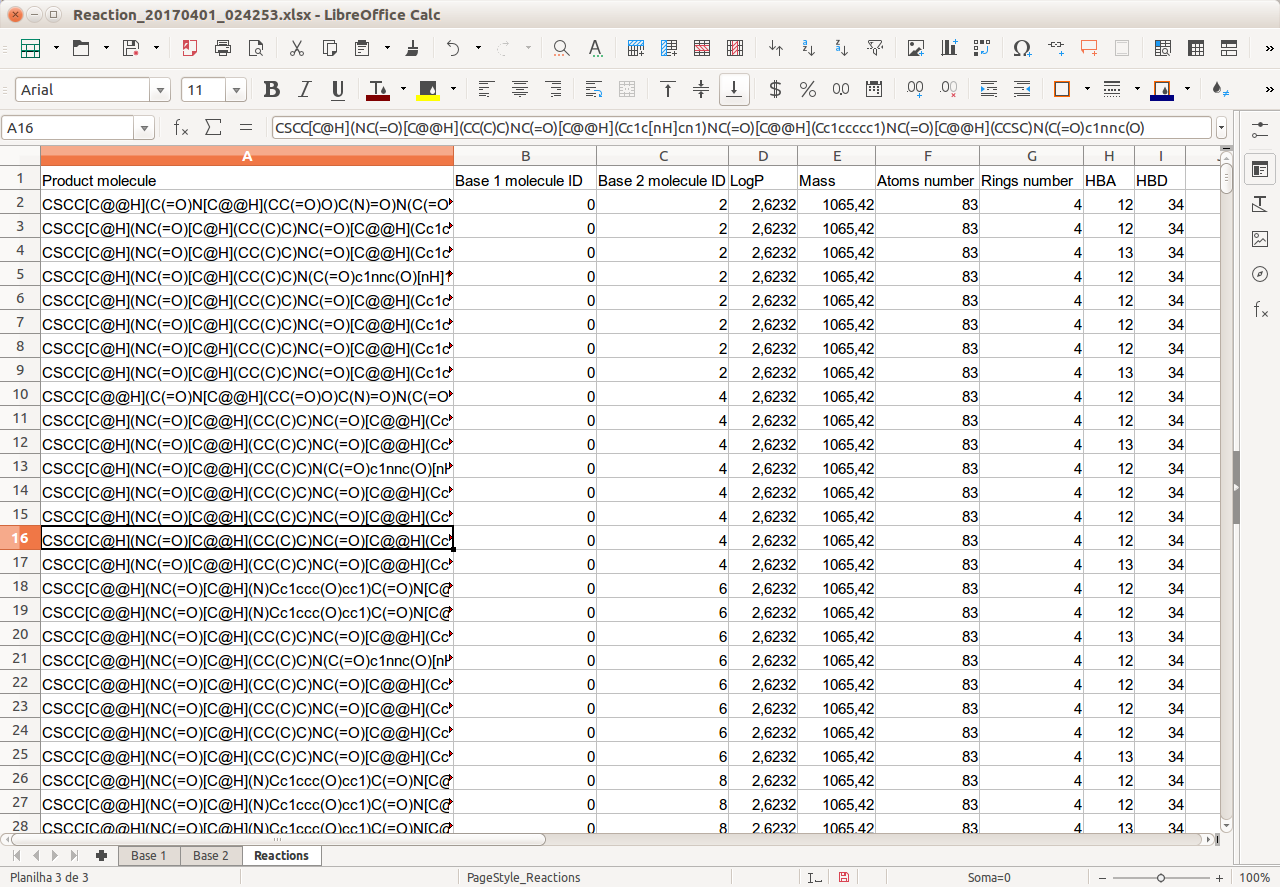
\includegraphics[scale=0.4]{reaction5}
  \caption{Planilha eletrônica com os resultados gerados pelas reações.}
  \label{fig:react5}
\end{figure}

\chapter{Conclusão}

Ao final de todo o desenvolvimento e diversos testes com o trabalho obtivemos um
resultado satisfatório conseguindo alcançar todos os resultados que planejamos.
O sistema está funcionando em produção e pode se acessado (temporariamente) no
endereço: \url{http://www.taiar.com.br/reactions}. Por enquanto a aplicação se encontra
em um servidor particular com baixos recursos, o que não nos permite, por exemplo,
reagir duas bases de compostos relativamente grandes ou operações mais pesadas envolvendo
bases de reagentes com muitos registros. Em breve existem planos de disponibilizar
o serviço em um servidor público e com infraestrutura apropriada para suportar todo
o tipo de operações.

Como mencionado anteriormente, existem ainda muitas funcionalidades a serem agregadas
ao primeiro protótipo que foi desenvolvido e já existe planejamento para que ele
seja mantido por alunos de pós-graduação da professora Rafaela. O código da implementação
da plataforma bem como instruções para colocá-la em funcionamento estão disponíveis
como um projeto open source em \url{https://github.com/taiar/bioapi-rails/} e toda
colaboração será bem vinda.

Algumas melhorias futuras que podem ser feitas no trabalho incluem:

\begin{itemize}
  \item possibilidade de reagir mais de duas bases simultaneamente;
  \item melhor visualização dos resultados tanto da filtragem quanto das reações;
  \item possibilidade de inputs de SMARTS por meio de desenho dos padrões buscados;
  \item possibilidade de fazer o input de reações;
  \item aumentar a gama de reações possíveis no sistema;
  \item ajustar melhor as reações aprimorando alguns parâmetros no RDKit.
\end{itemize}

O desenvolvimento do trabalho em si foi de grande satisfação pessoal e tanto pelo
seu bom andamento quanto pelo prazer de aprender uma área da computação na qual
eu ainda não havia entrado em contato. O trabalho de pesquisa para juntar as peças
que iam ao final compor o que havíamos vislumbrado foi um processo mais divertido
a cada nova descoberta.

\bibliography{monografia-andre_taiar}

\end{document}
